\clearpage
\section{Introduction}
\label{sec:Intro}

\textbf{Machine learning} is a field of artificial intelligence that uses statistical techniques to give a computer the ability to learn from data without being explicitly programmed to do so. 

\textbf{Genomics} is a branch of molecular biology concerned with the structure, function, evolution, and mapping of an organism's complete set of DNA.

In this project, we apply machine learning techniques to \textit{viral} genomic data recovered from human cells, and attempt to derive useful insights about the \textbf{EV-71 virus}, also known as hand-foot-and-mouth disease (HFMD).

\subsection{Machine Learning}

With the large volume of data available nowadays, it is impossible to apply statistical techniques and derive useful insights without making use of a computer. 

Considered one of the biggest innovations since the microchip, machine learning enables humans to build models and capture patterns within data. It allows one to define simple rules to improve the performance of these models. The applications of machine learning are manifold - from spam filters in e-mail to online banking, it is omnipresent. Machine learning's presence is growing, and its use cases continue increasing.

A machine learning model can be defined by its training data and the set of hypotheses functions.

Machine learning is broadly divided into the following 3 categories:-
\begin{itemize}
    \item Supervised Learning
    \item Unsupervised Learning
    \item Reinforcement Learning
\end{itemize}

In \textbf{supervised learning}, the training data are labelled, i.e. each data point is attached with its true value, or \textit{ground truth}. Typical problems include \textit{classification} (binary/multi-class) and \textit{regression}. E.g. If given a training dataset consisting of pictures of cats and dogs, our model accurately predicts whether a new image is that of a cat or a dog. This is a \textit{classification} problem. Another simple example is of a dataset with people's heights and weights. Given a new person's height, we should be able to accurately predict weight. This is a \textit{regression} problem.

In \textbf{unsupervised learning}, unlike supervised learning, the training data are unlabelled. The number of labels may or may not be specified beforehand. Unsupervised learning is commonly used as an initial exploratory technique to draw useful patterns from the dataset. E.g. Given many different books, classifying them into different categories, or \textit{clusters}, can help us identify the genres they belong to. 

\textbf{Reinforcement learning} is different from both supervised and unsupervised learning. It focuses on maximizing reward potential from the data by balancing the trade-off between exploration and exploitation. E.g. In recommendation engines, the items showed to a particular user may ordered based on how much they liked previous products or how \textit{different} they are from previous products. This is done to maximize the number of clicks, i.e. the \textit{reward}.

Since the data that we have in this project is unlabelled, our focus is on \textit{unsupervised learning}.

\subsection{Genomics}

Genomes contain the complete set of genes present in an organism, and genomics describe how genetic information is stored and interpreted in the cell.

\subsubsection{Key Definitions and Terms}
\begin{itemize}
    \item \textbf{Nucleobases}: Components of nucleotides, that are the building blocks of DNA - Adenine, Thymine, Cytosine, Guanine (A,T,C,G). Additionally, Uracil (U) is used instead of Thymine (T) for RNA.
    \item \textbf{Codons}: A sequence of three DNA or RNA nucleotides that corresponds with a specific amino acid or stop signal during protein synthesis. There are a total of 64 such codons, which map to 20 amino acids (and stop signals) through the \textit{genetic code}.
    \item \textbf{Amino acid}: Sequences of nucleotides that are the building blocks of proteins. There are 20 canonical amino acids.
    \item \textbf{DNA}: Deoxyribonucleic acid, a molecule shaped like a double helix, that contains the genetic material for all organisms on Earth (including viruses).
    \item \textbf{RNA}: Ribonucleic acid, a single helix, polymeric molecule that is essential in various biological roles in coding, decoding, regulation and expression of genes. Biologically active RNAs, including transport, ribosomal and small nuclear RNA (tRNA, rRNA, snRNAs) fold into unique structures guided by complementary pairing between nucleotide bases.
    Cellular organisms use messenger RNA (mRNA) nucleotides to direct synthesis of specific proteins.
    \item \textbf{Protein}: Sequences of amino acids that carry out the majority of cellular functions such as motility, DNA regulation, and replication.
    \item \textbf{Transcription}: The process in which a DNA sequence of a gene is rewritten, or \textit{transcribed}, to make an RNA molecule. (In eukaryotes, the RNA polymerase makes a strand of mRNA from DNA).
    \item \textbf{Translation}: The sequence of the mRNA is decoded, or \textit{translated}, to specify an amino acid sequence (i.e. protein).
    \item \textbf{Gene}: A region of DNA (deoxyribonucleic acid) coding either for the messenger RNA encoding the amino acid sequence in a polypeptide chain or for a functional RNA molecule.
    \item \textbf{Chromosome}: Cellular structures that contain genes. A chromosome comprises of a single DNA molecule that may be either circular or linear.
    \item \textbf{Virus}: A small infectious agent that replicates only inside the living cells of other organisms.
    \item \textbf{Gene Expression}: The generation of a functional gene product from the information encoded by a gene, through the processes of transcription and translation. Gene products are often proteins. \footnote{Non-protein coding genes can encode functional RNA, including ribosomal RNA (rRNA), transfer RNA (tRNA) or small nuclear RNA (snRNA)}
\end{itemize}

\subsubsection{Central Dogma}
\begin{figure}[h]
\centering
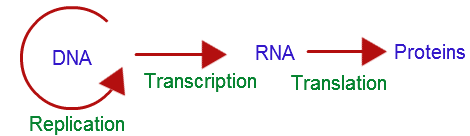
\includegraphics[width=0.5\textwidth]{Figures/central-dogma.png}
\caption{Central dogma of Molecular Biology}
\end{figure}

The central dogma of biology states that:
DNA is \textit{transcribed} by RNA polymerases into mRNA (messenger RNA), which is read by ribosomes to generate protein through \textit{translation}. \cite{crick1970central}

In this project, our focus is on translation. More formally, we will be studying the translational interaction between the EV-71 virus and its host cell, by observing gene expression values at different timepoints.

\subsubsection{Virus-Host Interaction}

When a host gets infected with a virus, the virus hijacks the host cell’s translation machinery, which affects protein production.

The viral replication process begins when a virus infects its host by attaching to the host cell and penetrating the cell wall or membrane. The viral genome then hijacks the host cell's translation mechanism, forcing it to replicate the viral genome by producing viral proteins to make new capsids (the protein shell of a virus that protects it). The viral particles are then assembled into new viruses. The new viruses burst out of the host cell during a process called lysis, killing the host cell. Some viruses take a portion of the host's membrane during the lysis process to form an envelope around the capsid. \cite{ScitableVirus}

Following viral replication, the new viruses may go on to infect new hosts. Many viruses cause diseases in humans, such as influenza, chicken pox, AIDS, the common cold, and rabies. 

\subsubsection{Objective}

Thus, when a virus infects a cell, most of the processes in the cell get shut down and some proteins don't get generated. There are groups of:-
\begin{enumerate}
    \item Genes that escape this shut down by the virus \label{imp}
    \item Genes that aid in the shut down
    \item Genes that are not influenced by the virus
\end{enumerate}

[\ref{imp}] is the most important, as these are the ones that the virus needs for its own production.

Thus, our objective is to identify these groups from the set of genes that we have available. We do this by using machine learning techniques on the genes and their expression data. 

\subsubsection{Hand-Foot-Mouth-Disease}

Hand, foot, and mouth disease (HFMD) is a common infection caused by a group of viruses. The one we will be examining in this report is the enterovirus 71, or the EV-71 virus. HFMD mostly affects small children, occasionally spreading to adults. It typically begins with a fever, which is followed by rashes and bumps on other parts of the body. Currently, there is no treatment that specifically targets the disease, and nor is there a vaccine that is approved for use in Singapore \cite{ang2009epidemiology}.

\subsection{Data Generation through Genome Sequencing Techniques}

RNA sequencing refers to techniques used to determine the sequence of RNA molecules. It includes high-throughput shotgun sequencing of cDNA molecules obtained by reverse transcription from RNA, and next-generation sequencing technologies to sequence the RNA molecules within a biological sample in an effort to determine the primary sequence and relative abundance of each RNA molecule.

For this project, we primarily use gene expression data that has been generated using the following techniques:-

\begin{itemize}
    \item \textbf{RNASeq}: RNASeq uses next-generation sequencing (NGS) to reveal the presence and total quantity of RNA in a biological sample at a given moment.
    \item \textbf{Ribosome Profiling (RPF)}: RPF uses specialized messenger RNA (mRNA) sequencing to determine which mRNAs are being actively translated. Unlike RNASeq, which sequences all of the mRNA of a given sequence present in a sample, RPF only targets mRNA sequences that are being actively translated.
\end{itemize}


